% CAP description for Figure Canvas
\begin{itemize}
\item  The figure canvas (\bxfigref{figurecanvas}) is an editor where figures, connections and anchors are displayed. 

\begin{figure}
\begin{center}
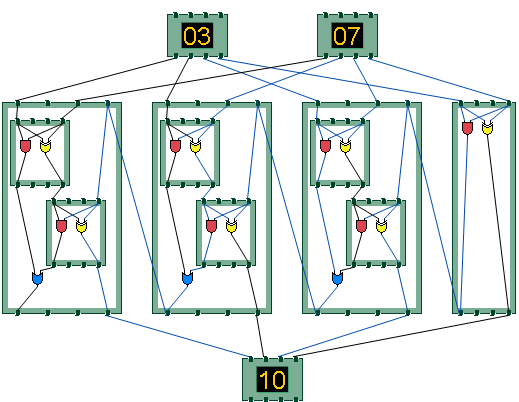
\includegraphics{PS/FigureCanvas}
\caption{Figure Canvas}
\label{figurecanvas}
\end{center}
\end{figure}

\item Testing GEF components  involves mapping this figure canvas and locating the figures based on their textpath. 
\item Use the GEF \gdinspector{} to find out the textpath of the figures in the canvas \bxextref{\gduserman}{user,TasksInspectorGEF}. 
\item The figure canvas itself contains various items which can be addressed. 
\item Individual figures (\bxfigref{figure}).

\begin{figure}
\begin{center}
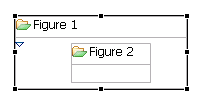
\includegraphics{PS/Figure}
\caption{A selected figure containing another figure}
\label{figure}
\end{center}
\end{figure}

\item Tools (\bxfigref{tools}).

\begin{figure}
\begin{center}
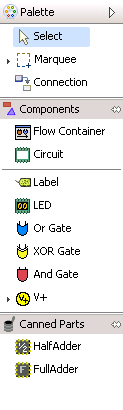
\includegraphics{PS/Tools}
\caption{Various tools on the palette}
\label{tools}
\end{center}
\end{figure}

\item Connections (\bxfigref{connection}).

\begin{figure}
\begin{center}
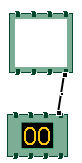
\includegraphics{PS/Connection}
\caption{A connection between two figures}
\label{connection}
\end{center}
\end{figure}

\item Connection anchors. These are the points where connections join to figures. Connection anchors are considered as figures. As such, they can be addressed (clicked, checked etc) using a textpath. 
\end{itemize}

\clearpage
